\documentclass{ctexart}
\usepackage{palatino}
\usepackage{tikz}
\usetikzlibrary{shapes.geometric, arrows}
\usepackage{bm}
\usepackage{geometry}
\usepackage{titlesec} %自u格式的宏包
\usepackage{picinpar,graphicx}
\usepackage{zhnumber}
\usepackage{float}
\usepackage{caption,subcaption}
\usepackage{amsmath}
\usepackage{amssymb}
\usepackage{fancyhdr}%页眉页脚
\usepackage{multirow}
\usepackage{upgreek}
\usepackage{paralist}
\usepackage{diagbox,array}
\usepackage{cite}
\usepackage{minted}
\usepackage{listings}
\usepackage{xcolor}
\usepackage{hyperref}
\usepackage{tabularx}
\usepackage{booktabs}
\usepackage{fancyhdr}
\usepackage{verbatim}
\usepackage{supertabular}
\usepackage{subfiles}
\usepackage{siunitx} 
\usepackage{multicol}
\usepackage{enumitem}
%\usepackage{pgfplots} 
\usepackage{circuitikz}
\usetikzlibrary{arrows.meta, positioning, shapes.symbols}
\usepackage{hologo}
\usepackage[super]{gbt7714}


\newCJKfontfamily{\cusong}[AutoFakeBold={2.17}]{SimSun}
\newCJKfontfamily{\cuhei}[AutoFakeBold={3.17}]{SimHei}
\geometry{a4paper,left=0.75in,right=0.75in,top=1in,bottom=1in} %页边距

\lstset{
	basicstyle=\ttfamily, % 设置字体族
	breaklines=true, % 自动换行
	keywordstyle=\bfseries, % 设置关键字为粗体，颜色为 NavyBlue
	morekeywords={}, % 设置更多的关键字，用逗号分隔
	emph={self}, % 指定强调词，如果有多个，用逗号隔开
	emphstyle=\bfseries\color{Rhodamine}, % 强调词样式设置
	commentstyle=\itshape\color{black!50!white}, % 设置注释样式，斜体，浅灰色
	%stringstyle=\bfseries\color{PineGreen!90!black}, % 设置字符串样式
	columns=flexible,
	numbers=left, % 显示行号在左边
	numbersep=2em, % 设置行号的具体位置
	numberstyle=\footnotesize % 缩小行号
}


\counterwithin{figure}{section}
\counterwithin{table}{section}
\counterwithin{equation}{section}

\renewcommand{\thefigure}{ \arabic{section}-\arabic{figure}}
\renewcommand{\theequation}{ \arabic{section}-\arabic{equation}}
\renewcommand{\thetable}{ \arabic{section}-\arabic{table}}
\renewcommand \thesubsection {\arabic{section}.\arabic{subsection}.}
\renewcommand \thesection {第\zhnum{section}章}
\renewcommand \thesubsubsection{\arabic{section}.\arabic{subsection}.\arabic{subsubsection}.}
\renewcommand{\caption}[1]{\caption[\songti\ziju{-5}]{#1}}
%\\totalnumber{10}
\renewcommand{\thesubfigure}{\arabic{subfigure}}

\titleformat{\section}[block]{\songti\zihao{-4}}{项目作业\arabic{section}：}{0em}{}[]
\titleformat{\subsection}[block]{\songti\zihao{-4}\linespread{1}}{\quad\arabic{subsection}）}{1em}{}[]
\titleformat{\subsubsection}[block]{\songti\zihao{-4}\linespread{1}}{\quad\roman{subsubsection}}{1em}{}[]
\titleformat{\paragraph}[block]{\songti\zihao{-4}}{(\arabic{paragraph})}{1em}{}[]

\setlength{\baselineskip}{20pt}


\pagenumbering{arabic}

\setlength{\parskip}{0.1pt}


\pagestyle{fancy}%清除原页眉页脚样式
\fancyhf{} 
%\thispagestyle{empty}
\renewcommand\headrulewidth{0pt} 
%\rhead[C]{\centering \zihao{5} \songti 传感器与单片机应用综合实践\quad\quad 课程设计说明书}
\rfoot[C]{\thepage}


\makeatletter
\def\@cite#1#2{\textsuperscript{[#1\if@tempswa, #2\fi]}}
\makeatother

\begin{document}
	\section{线性卷积}
		\subsection{题目}
			编写序列起点不在零点时的卷积程序。任选两序列（起点不在零点）用所学列表法或作图法计算以下两序列卷积，并用程序验证，并与序列起点在零点时的结果对比。
		\subsection{分析}
			本题选用《信号处理原理与运用》P63的题目3-7的两个序列$h(n)$和$x(n)$，其波形如图\ref{fig:第一问选用序列}所示。其中输入序列$x(n)$的起点为$n=-2$，满足题中起点不在零点的要求。\par
			首先使用列表法进行线性卷积求解，随后使用Mworks进行程序验证。\par
			在Mworks中使用线性卷积函数conv()即可得到两个序列的线性卷积值，但是Mworks中序列起点硬性规定为0，因此需要将Mworks的计算结果作相应的移动。
			\begin{figure}[h]
				\subcaptionbox{线性时不变系统的单位脉冲函数$h(n)$}[0.5\textwidth]{
					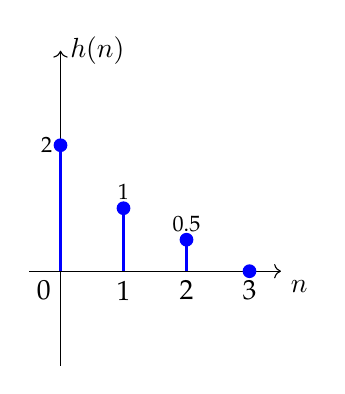
\begin{tikzpicture}[scale=0.8] % 调整 scale 控制子图大小
						\draw[->] (-0.5,0) -- (3.5,0) node[below right] {$n$};
						\draw[->] (0,-1.5) -- (0,3.5) node[right] {$h(n)$};
						
						\draw[blue, thick](0,0) -* (0,2) node[black,left,scale=0.8]{2};
						\draw[blue, thick](1,0) -* (1,1)node[black,above,scale=0.8]{1};
						\draw[blue, thick](2,0) -* (2,0.5)node[black,above,scale=0.8]{0.5};
						
						\filldraw[draw=blue,fill=blue] (0,2) circle (0.1);
						\filldraw[draw=blue,fill=blue] (1,1) circle (0.1);
						\filldraw[draw=blue,fill=blue] (2,0.5) circle (0.1);
						\filldraw[draw=blue,fill=blue] (3,0) circle (0.1);
						
						\node at (0,0) [below left] {0};
						\node at (1,0) [below] {1};
						\node at (2,0) [below] {2};
						\node at (3,0) [below] {3};
					\end{tikzpicture}
				}
				\subcaptionbox{输入序列$x(n)$}[0.5\textwidth]{
					\begin{tikzpicture}[scale=0.8]
						\draw[->] (-2.5,0) -- (3.5,0) node[below right] {$n$};
						\draw[->] (0,-1.5) -- (0,3.5) node[right] {$x(n)$};
						
						\draw[blue, thick](-2,0) -* (-2,-1) node[black,left,scale=0.8]{-1};
						\draw[blue, thick](1,0) -* (1,1)node[black,above,scale=0.8]{1};
						\draw[blue, thick](3,0) -* (3,2)node[black,above,scale=0.8]{2};
						
						\filldraw[draw=blue,fill=blue] (-2,-1) circle (0.1);
						\filldraw[draw=blue,fill=blue] (-1,0) circle (0.1);
						\filldraw[draw=blue,fill=blue] (0,0) circle (0.1);
						\filldraw[draw=blue,fill=blue] (1,1) circle (0.1);
						\filldraw[draw=blue,fill=blue] (2,0) circle (0.1);
						\filldraw[draw=blue,fill=blue] (3,2) circle (0.1);
						
						\node at (-2,0)[above] {-2};
						\node at (-1,0)[below] {-1};
						\node at (0,0) [below left] {0};
						\node at (1,0) [below] {1};
						\node at (2,0) [below] {2};
						\node at (3,0) [below] {3};
					\end{tikzpicture}
				}
				\caption{第一问选用序列}
				\label{fig:第一问选用序列}
			\end{figure}
		\subsection{列表法计算}
			\begin{table}[!ht]
				\centering
				\caption{第一问列表法求解表格}
				\label{tab:第一问列表法求解表格}
				\begin{tabular}{|c||c|c|c|c|c|c|c|c|c|c||c|}
					\hline
					$m$ & -4 & -3 & -2 & -1 & 0 & 1 & 2 & 3 & 4 & ~ &   \\ \hline
					$x(m)$ & ~ & ~ & -1 & 0 & 0 & 1 & 0 & 2 & ~ & ~ &   \\ \hline
					$h(m)$ & ~ & ~ & ~ & ~ & 2 & 1 & 0.5 & ~ & ~ & ~ &   \\ \hline\hline
					$h(-m)$ & ~ & ~ & 0.5 & 1 & 2 & ~ & ~ & ~ & ~ & ~ & $y(0)=-0.5$  \\ \hline
					$h(1-m)$ & ~ & ~ & ~ & 0.5 & 1 & 2 & ~ & ~ & ~ & ~ & $y(1)=2$  \\ \hline
					$h(2-m)$ & ~ & ~ & ~ & ~ & 0.5 & 1 & 2 & ~ & ~ & ~ & $y(2)=1$  \\ \hline
					$h(3-m)$ & ~ & ~ & ~ & ~ & ~ & 0.5 & 1 & 2 & ~ & ~ & $y(3)=4.5$  \\ \hline
					$h(4-m)$ & ~ & ~ & ~ & ~ & ~ & ~ & 0.5 & 1 & 2 & ~ & $y(4)=2$  \\ \hline
					$h(5-m)$ & ~ & ~ & ~ & ~ & ~ & ~ & ~ & 0.5 & 1 & 2 & $y(5)=1$  \\ \hline
					$h(-1-m)$ & ~ & 0.5 & 1 & 2 & ~ & ~ & ~ & ~ & ~ & ~ & $y(-1)=-1$  \\ \hline
					$h(-2-m)$ & 0.5 & 1 & 2 & ~ & ~ & ~ & ~ & ~ & ~ & ~ & $y(-2)=-2$  \\ \hline
				\end{tabular}
			\end{table}\par
			最终得到的线性卷积结果为$y(n)=[-2,-1,-0.5,2,1,4.5,2,1]$
		\subsection{代码}
			\begin{lstlisting}[language=Python]
using TyMath        # 调用同元数学库
h = [2,1,0.5,0]     # 有限序列h(n)
x = [-1,0,0,1,0,2]  # 有限序列x(n)
y = conv(x,h)       # y(n)为x(n)和h(n)的线性卷积
print(y)            # 输出线性卷积序列y(n)
			\end{lstlisting}
		\subsection{运行结果}
			\begin{figure}[h]
				\centering
				\begin{subfigure}{\linewidth}
					\centering
					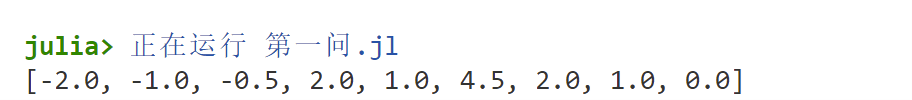
\includegraphics[width=0.75\linewidth]{./图片/第一问}
				\end{subfigure}
				\caption{序列卷积结果}
				\label{fig:序列卷积结果}
			\end{figure}
		\subsection{结论}
			通过对比，易知无论序列起点是否在零点，卷积的数值结果相同。而卷积结果的起始位置为两序列起点之和，所以起点不同时会造成结果的位置偏移。卷积运算的数值结果由序列元素决定，而结果的时序位置由两序列的起点共同决定。实际应用中，若忽略起点信息，虽然数值正确，但可能导致时间序列错位。
			
	\newpage		
	\section{系统的作用}
		\subsection{题目}
			设某系统单位冲激响应为$h(n)=a^nu(n)$,$\lvert a\rvert<1$；画出不同$a$值下$h(n)$及$y(n)=h(n)*x(n)$的波形。其中$x(n)$为某指数1993年-2014年的月度收盘数据（见Excel表并截取数据导入MATLAB）；根据结果论述该系统的作用。
		\subsection{分析}
			首先需要将给出的Excel进行整理，只保留年份为1993年-2014年的月度收盘数据。以此得到两列有效数据。随后将其转为CSV格式。最后根据题目要求，给出相应代码。
		\subsection{代码}
			\begin{lstlisting}[language=Python]
using TyBase        # 调用同元基础库
using TyMath        # 调用同元数学库
using TyPlot        # 调用同元绘图库
using CSV           # 调用CSV读取库

file_path = joinpath(@__DIR__, "某指数月度历史数据.csv") # 生成文件绝对路径
table = DataFrame(CSV.File(file_path));                # 读取表格
x = table[:,2]                  # 取出文件第二列作为有限序列x(n) 

for i in 1:9                               # 共绘制9幅图
	subplot(3,3,i)                      # 第i张图绘制在3行3列的第i个位置
	a=i*0.2-1                           # 第i张图取对应a值（相当于a=-0.8:0.2:0.8）
	y=shock_response(a,x)               # 调用响应解算函数shock_response（）
	plot(y)                             # 绘制响应曲线
	title("a="*@sprintf("%.1f", a))     # 生成图名
end

function shock_response(a::Float64,x::Vector)    # 定义响应解算函数
	h=zeros(length(x))                        # 定义冲激响应h(n)的长度
	for i in 1:length(x)                      # 求解h(n)
		h[i]=power(a,i)                         
	end
	return conv(h,x)                          # 返回卷积结果
end
			\end{lstlisting}
		\subsection{运行结果}
			\begin{figure}[H]
				\centering
				\begin{subfigure}{\linewidth}
					\centering
					
\includegraphics[width=0.75\linewidth]{./图片/第二问}
				\end{subfigure}
				\caption{不同$a$值下对应响应曲线}
				\label{fig:不同值下对应响应曲线}
			\end{figure}
		\subsection{结论}
			该系统的单位冲激响应为$h(n)=a^nu(n)$，其中a是一个小于1的常数。\par
			根据差分方程的定义，单位冲激响应描述了系统对一个单位冲激信号的响应。在这种情况下，当输入信号为单位冲激函数$u(n)$时，系统的输出为$h(n)$。\par
			由于a的取值范围为$\lvert a\rvert<1$，可以发现随着$n$的增加，$a^n$的值会逐渐减小，并趋近于0。而$u(n)$表示输入信号在$n$大于等于$0$时为$1$，小于$0$时为$0$。因此，$h(n)$在$n$大于等于$0$时始终存在，并且随着$n$的增加而逐渐减小。\par
			根据图2-1中的波形图结果进行比较分析，输入不同的a值，我们可以观察到系统的输出信号$y(n)$的变化。当$\lvert a\rvert<1$时，系统是一个低通滤波器。当$a$越接近$1$时，输出信号$y(n)$对输入信号$x(n)$的高频成分有更强的抑制作用，即更加平滑。当a越接近0时，输出信号$y(n)$对输入信号$x(n)$的低频成分也会被抑制，即更加锐化。\par
			该系统的作用类似于低通滤波器，可以用来平滑信号、降低噪声、滤除高频干扰等。它能够使输入信号的高频成分衰减，并保留输入信号的低频成分。这在很多实际应用中都是非常有用的，比如音频处理、图像处理、通信系统等。\par
			总结起来，它的作用是对输入信号进行低通滤波，通过抑制高频成分而保留低频成分，从而实现对输入信号进行平滑处理或锐化处理的效果，具体效果取决于$a$值的选择。\par
	
	\newpage
	\section{循环卷积}
		\subsection{题目}
			完成序列的循环移位运算与$L$点循环卷积（可以用Toeplitz函数编写循环移位矩阵）运算，并与线性卷积结果作比较，分析运算结果。
		\subsection{分析}
			本题选用《信号处理原理与运用》P112的题目4-14的两个序列$x(n)$和$h(n)$，其波形如图\ref{fig:第三问选用序列}所示。\par
			在Mworks中使用线性卷积函数conv()即可得到两个序列的线性卷积值，使用循环卷积函数cconv()即可得到两个序列的循环卷积值。
			\begin{figure}[h]
				\subcaptionbox{有限序列$x(n)$}[0.5\textwidth]{
					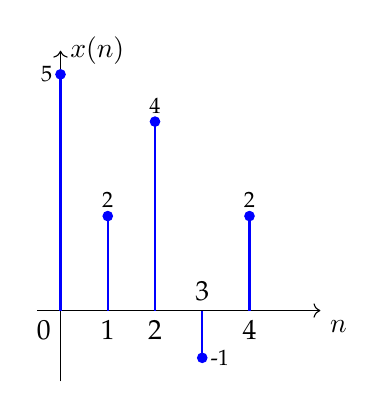
\begin{tikzpicture}[scale=0.6]
						\draw[->] (-0.5,0) -- (5.5,0) node[below right] {$n$};
						\draw[->] (0,-1.5) -- (0,5.5) node[right] {$x(n)$};
						
						\draw[blue, thick](0,0) -* (0,5) node[black,left,scale=0.8]{5};
						\draw[blue, thick](1,0) -* (1,2) node[black,above,scale=0.8]{2};
						\draw[blue, thick](2,0) -* (2,4) node[black,above,scale=0.8]{4};
						\draw[blue, thick](3,0) -* (3,-1) node[black,right,scale=0.8]{-1};
						\draw[blue, thick](4,0) -* (4,2) node[black,above,scale=0.8]{2};
						
						\filldraw[draw=blue,fill=blue] (0,5) circle (0.1);
						\filldraw[draw=blue,fill=blue] (1,2) circle (0.1);
						\filldraw[draw=blue,fill=blue] (2,4) circle (0.1);
						\filldraw[draw=blue,fill=blue] (3,-1) circle (0.1);
						\filldraw[draw=blue,fill=blue] (4,2) circle (0.1);
						
						\node at (0,0) [below left] {0};
						\node at (1,0) [below] {1};
						\node at (2,0) [below] {2};
						\node at (3,0) [above] {3};
						\node at (4,0) [below] {4};
					\end{tikzpicture}
				}
				\subcaptionbox{有限序列$h(n)$}[0.5\textwidth]{
					\begin{tikzpicture}[scale=0.6]
						\draw[->] (-0.5,0) -- (3.5,0) node[below right] {$n$};
						\draw[->] (0,-3.5) -- (0,4.5) node[left] {$h(n)$};
						
						\draw[blue, thick](0,0) -* (0,-3) node[black,left,scale=0.8]{-3};
						\draw[blue, thick](1,0) -* (1,4)node[black,right,scale=0.8]{4};
						\draw[blue, thick](2,0) -* (2,-1)node[black,below,scale=0.8]{-1};
						
						\filldraw[draw=blue,fill=blue] (0,-3) circle (0.1);
						\filldraw[draw=blue,fill=blue] (1,4) circle (0.1);
						\filldraw[draw=blue,fill=blue] (2,-1) circle (0.1);
						
						
						\node at (0,0) [below left] {0};
						\node at (1,0) [below] {1};
						\node at (2,0) [above] {2};
					\end{tikzpicture}
				}
				\caption{第三问选用序列}
				\label{fig:第三问选用序列}
			\end{figure}
		\subsection{代码}
			\begin{lstlisting}[language=Python]
using TyMath                # 调用同元数学库
using TyPlot                # 调用同元绘图库
using TySignalProcessing    # 调用同元信号处理库

x = [5,2,4,-1,2]    # 有限序列x(n)
h = [-3,4,-1]       # 有限序列h(n)

subplot(2,2,1)
y = conv(x,h)      # y(n)为x(n)和h(n)的线性卷积
stem(y)            # 输出线性卷积序列y(n)
title("线性卷积")

subplot(2,2,2)
y = cconv(x,h,6)   # y(n)为x(n)和h(n)的6点循环卷积
stem(y)            # 输出6点循环卷积序列y(n)
title("6点循环卷积")

subplot(2,2,3)
y = cconv(x,h,7)   # y(n)为x(n)和h(n)的7点循环卷积
stem(y)            # 输出7点循环卷积序列y(n)
title("7点循环卷积")

subplot(2,2,4)
y = cconv(x,h,8)   # y(n)为x(n)和h(n)的8点循环卷积
stem(y)            # 输出8点循环卷积序列y(n)
title("8点循环卷积")
			\end{lstlisting}
		\subsection{运行结果}
			\begin{figure}[H]
				\centering
				\begin{subfigure}{\linewidth}
					\centering
					
\includegraphics[width=0.55\linewidth]{./图片/第三问}
				\end{subfigure}
				\caption{线性卷积与循环卷积运行结果}
				\label{fig:线性卷积与循环卷积运行结果}
			\end{figure}
		\subsection{结论}
			线性卷积是时域中两个离散序列的卷积运算，结果长度等于两序列长度之和减$1$（即$N+M-1$）。计算过程为：反转其中一个序列后滑动，逐点相乘并求和。公式如下：
			\begin{gather}
				y(n)=x(n)*h(n)=\sum_{m=-\infty}^{+\infty}x(m)h(n-m)
			\end{gather}\par
			循环卷积基于周期性假设，将序列视为周期为$L$的信号，通过圆周移位后相乘求和。结果长度固定为$L$。若$L\leq N+M−1$，循环卷积等于线性卷积补零到 $L$点；$L<N+M−1$，则会发生混叠。公式如下：
			\begin{gather}
				y(n)=x(n)\otimes h(n)=\sum_{m=0}^{N-1}x(m)h((n-m))_NR_N(n)
			\end{gather}\par
			通过图\ref{fig:线性卷积与循环卷积运行结果}中的四张图对比可知：$7$点循环卷积与线性卷积的结果相同；$6$点循环卷积会发生混叠现象，将最后一个点的值加到第一个点上去了；8点循环卷积为线性卷积结果后补一个零。\par
			由此可知，当$L \geq N+M−1$时，循环卷积与线性卷积数值相同，仅时间轴补零扩展。若当$L<N+M−1$，循环卷积结果因混叠失真。
			
	\newpage
	\section{频域求解线性卷积}
		\subsection{题目}
			利用FFT及IFFT求解LSI系统输出$y[n]=x[n]*h[n]$，并用时域线性卷积验证。输入与单位采样响应可以自己设。
		\subsection{分析}
			本题选用《信号处理原理与运用》P63的题目3-7的两个序列$h(n)$和$x(n)$，其波形如图\ref{fig:第一问选用序列}所示。\par
			在Mworks中使用线性卷积函数conv()即可得到两个序列的线性卷积值，使用快速傅里叶变换及逆变换函数fft()和ifft()即可得到两个序列的变换值。
		\subsection{代码}
			\begin{lstlisting}[language=Python]
using TyMath
using TyPlot

h = [2,1,1,0]     # 有限序列h(n)
x = [-1,0,0,1,0,2]  # 有限序列x(n)

####################线性卷积####################
y = conv(x,h)       # y(n)为x(n)和h(n)的线性卷积

subplot(1,2,1)      # 绘制散点图
stem(y)
title("直接线性卷积")

####################频域求解线性卷积####################
len = 16            # 补为16点，符合基2FFT
h=vcat(h,zeros(len-length(h)))
x=vcat(x,zeros(len-length(x)))

h_s = fft(h)        # 快速傅里叶FFT
x_s = fft(x)

y_s = h_s .* x_s    # 时域卷积等价于频域相乘
y = ifft(y_s)       # 反快速傅里叶IFFT

subplot(1,2,2)      # 绘制散点图
stem(y)
title("频域求解线性卷积")
			\end{lstlisting}
		\subsection{运行结果}
			\begin{figure}[H]
				\centering
				\begin{subfigure}{\linewidth}
					\centering
					
\includegraphics[width=0.55\linewidth]{./图片/第四问}
				\end{subfigure}
				\caption{时域直接卷积结果及频域 FFT/IFFT 求解结果}
				\label{fig:时域直接卷积结果及频域 FFT/IFFT 求解结果}
			\end{figure}
		\subsection{结论}
			在不进行零填充的情况下，conv(x,h)得到的线性卷积长为$6+4−1=9$点，序列为$y(n)=x(n)*h(n)=[-2,-1,-1,2,1,2,0,0,0]$。在频域方法中，将$x$、$h$都零填充到$16$点，然后对它们分别做FFT，相乘后再做IFFT，得到的序列$y_f$也是$16$点长。将前$9$点信号截取出来，可以与上述时域卷积结果精确对应。对比两种方法得到的前$9$点序列，可见它们在每一点上完全相同，验证了时域卷积与频域 FFT/IFFT 求解的等价性。\par
			FFT本质上执行的是循环卷积。若直接对原始长度$6$点和$4$点序列做 FFT，相乘后再 IFFT，结果将产生“时间上环绕”的叠加，与线性卷积不同。为了让循环卷积等同于线性卷积，需将两序列长度都补到至少$6+4−1=9$或更大的二次幂（如取$16$点），这样在 IFFT 时循环卷积不会出现重叠部分，前$9$点恰好就是完整的线性卷积结果。\par
			本题通过仿真验证了线性时域卷积$y(n)=x(n)*h(n)$与离散傅里叶变换后在频域相乘再做逆变换的过程等价。通过对信号进行足够的零填充，可消除循环卷积带来的混叠。在数字信号处理中，FFT/IFFT，方法能降低复杂度，零填充也为快速卷积提供了灵活性：可按需选择FFT长度（一般取大于等于$L_x+L_h-1$的最小二次幂）。另外，零填充长度不足或未取二次幂都可能导致频域卷积结果与线性卷积不符。
			
	\newpage
	\section{验证时域采样定理}
		\subsection{题目}
			对正弦信号以不同采样频率进行采样，分析不同采样率下信号频谱，验证采样定理，并对谱线进行说明。（信号自己设定）
		\subsection{分析}
			本题对频率$f_0=10$Hz的正弦信号$y=\sin20\pi t$进行不同采样频率采样。采样时长$T_p$设置为10。\par
			为了满足基2的快速傅里叶变换（FFT），频域采样点数$N$设为$2^{i+1}$，其中$i\in\mathbb{R}$。因此根据公式$T_p=NT$，时域采样间隔$T=\frac{10}{2^{i+1}}$，时域采样频率则为$f_s=\frac{1}{T}=\frac{2^{i+1}}{10}$。\par
			频率采样间隔满足公式$F=\frac{1}{T_P}=\frac{1}{10}$。根据奈奎斯特-香农采样定理（Nyquist–Shannon sampling theorem）：如果一个系统以超过信号最高频率至少两倍的速率对模拟信号进行均匀采样，那么原始模拟信号就能从采样产生的离散值中完全恢复。时域采样信号频率$f_s\geq2f_0$才能还原原始信号的频段。也就是$f_s\geq2\times10=20$Hz，此时采样点数$N=f_sT_p\geq20\times10=100$。
		\subsection{代码}
			\begin{lstlisting}[language=Python]
using TyBase
using TyMath
using TyPlot

for i in 1:9            # 共绘制9幅图（数据时间长度Tp不变，皆为10）
	T=10/power(2,i+1)   # 计算第i张图的时域采样间隔为T
	t=0:T:10            # 计算各个采样点时间
	y=sin.(20*pi*t)     # 计算各个采样点采样值
	y_s=fft(y)          # 快速傅里叶变换FFT
	y_s=y_s[1:power(2,i)]       # 去除周期延拓信号
	f=0:(1/10):(power(2,i)/10)-1/10  #得到频率坐标轴
	
	subplot(3,3,i)      # 绘图
	plot(f,abs.(y_s))
	title("采样频率fs="*@sprintf("%.1f",power(2,i+1)/10))
end
			\end{lstlisting}
		\subsection{运行结果}
			图\ref{fig:正弦信号在不同采样率下的频谱图}为代码的运行结果。\par
			当$f_s<2f_0=20$Hz时，主峰完全折叠，这四幅图上的最高谱线都不在$10$Hz，而是在$f=\lvert f_0−kf_s \rvert$附近，显然远低于奈奎斯特频率，信号已完全丧失原始频率信息。$fs=6.4 Hz$时，折叠成$\lvert10−2×6.4\rvert=2.8 $Hz，在图上可看见$2.8$Hz峰。虽然折叠位置逐渐向高频逼近，但仍然不在$10$Hz。第6次采样率仍未达到20 Hz，依然出现混叠。\par
			当到达临界采样率时，虽然取的采样率中没有恰好$20$Hz的图，但从$12.8$到$25.6$Hz 的过渡可见，混叠峰由 $2.8$ Hz 突然移向主频 $10$ Hz。从$f_s=25.6 Hz$起，主峰便固定出现在 $10 $Hz。\par
			当$f_s>20$ Hz时，每幅图上唯一且最显著的谱线都恰在$ 10$ Hz。理论上还应在$fs−10$ Hz处出现同样幅度的镜像峰，但由于我们只截取了“正频率”半谱，这些镜像峰都落在半谱之外，因此图中看不到。满足奈奎斯特采样定理后，频谱中仅存真实信号成分，无任何混叠假峰。\par
			\begin{figure}[H]
				\centering
				\begin{subfigure}{\linewidth}
					\centering
					
\includegraphics[width=0.75\linewidth]{./图片/第五问}
				\end{subfigure}
				\caption{正弦信号在不同采样率下的频谱图}
				\label{fig:正弦信号在不同采样率下的频谱图}
			\end{figure}
		\subsection{结论}
			只有当采样频率$f_s$大于信号最高频率两倍时，采样后的频谱中才会在原始频率处出现唯一且不被混叠的主峰。低于该阈值时，信号成分会被折叠到其他频率，导致失真不可恢复。当$f_s<2f_0$时，原频率$f_0$被映射到$f=\lvert f_0−kf_s \rvert$位置，出现虚假谱峰。一旦满足 $f_s>2f_0$，频谱中仅存真实信号成分，镜像谱峰移至采样带宽之外，不在可观测半谱内。频谱分辨率$\Delta f=\frac{1}{T_p}$由记录总时长$T_p$决定。
	
	\newpage
	\section{频谱泄漏的本质}
		\subsection{题目}
			$x_1$和$x_2$两模拟周期信号频率$f_1=20$Hz,$f_2=25$Hz,采样频率$f_s=100$Hz，分析不同采样点数（整周期、非整周期）下两信号的频谱，画出时频图，讨论频谱泄漏与周期截取的关系。
		\subsection{代码}
			\begin{lstlisting}[language=Python]
using TyBase
using TyMath
using TyPlot

# 定义处理函数cul_fft，采样信号频率frq，总采样时长T
function cul_fft(frq,T)
	t_f=1/100               # 采样间隔0.01秒
	t=0:t_f:T               # 生成采样点
	y=sin.(frq*2*pi*t)      # 对信号采样
	y_s=fft(y)              # 快速傅里叶变换
	y_s=y_s[1:div(length(y_s),2)]   # 去除周期延拓信号
	return y_s              # 返回频谱
end

####  采样时长为4秒的整周期采样  ####
subplot(1,2,1)              # 绘制子图1
plot(abs.(cul_fft(20,4)))   # 绘制20Hz频谱，采样4秒的频谱
hold("on")                  # 保留曲线
plot(abs.(cul_fft(25,4)))   # 绘制25Hz频谱，采样4秒的频谱
title("整周期采样频谱")

####  采样时长为4.2秒的非整周期采样  ####
subplot(1,2,2)              # 绘制子图2
plot(abs.(cul_fft(20,4.02)))# 绘制20Hz频谱，采样4.02秒的频谱
hold("on")                  # 保留曲线
plot(abs.(cul_fft(25,4.02)))# 绘制25Hz频谱，采样4.02秒的频谱
title("整周期采样频谱")
			\end{lstlisting}
		\subsection{运行结果}
			\begin{figure}[H]
				\centering
				\begin{subfigure}{\linewidth}
					\centering
					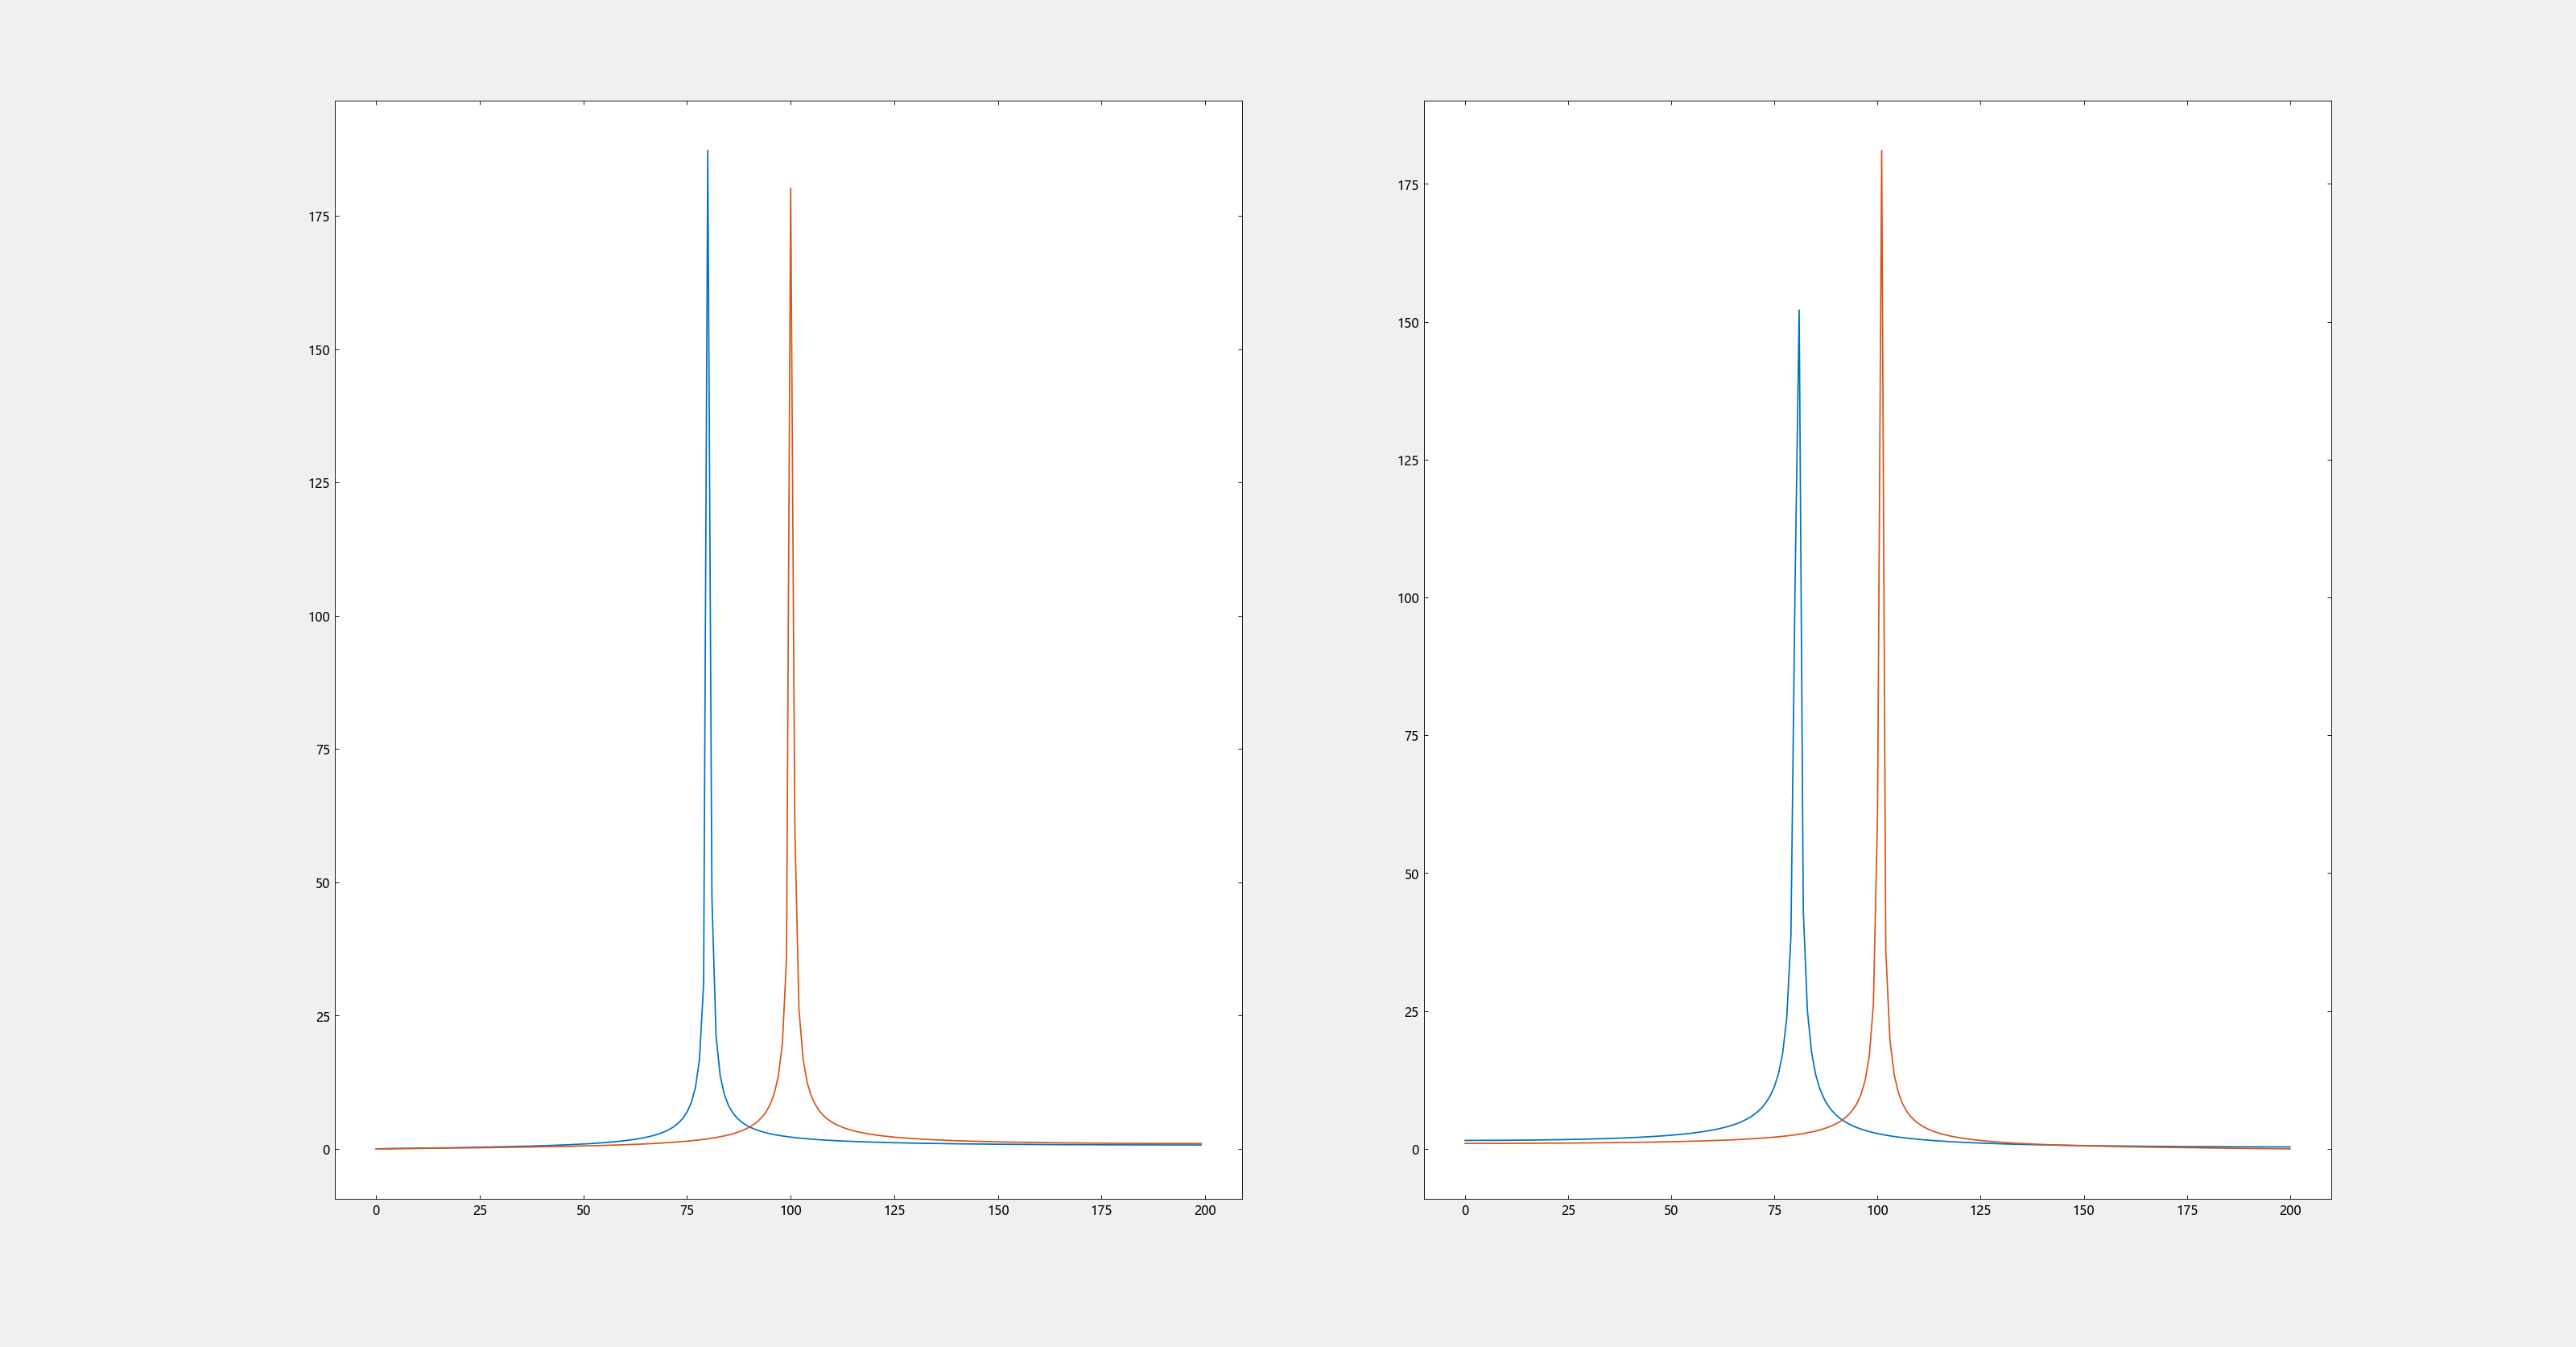
\includegraphics[width=0.75\linewidth]{./图片/第六问}
				\end{subfigure}
				\caption{整周期与非整周期采样频谱}
				\label{fig:整周期与非整周期采样频谱}
			\end{figure}
		\subsection{结论}
			\subsubsection{整周期截取与频谱特性}
			X1（20Hz）：每个周期对应采样点数 $N_1 = f_s/f_1 = 100/20 = 5$。若采样点数为5的整数倍，则频谱能量集中在20Hz处，无泄漏。\par
			X2（25Hz）：每个周期对应采样点数 $N_2 = f_s/f_2 = 100/25 = 4$。若采样点数为4的整数倍，频谱能量集中在25Hz处，无泄漏。\par
			同时满足整周期：当采样点数N为5和4的公倍数（如N=20）时，两信号均无泄漏。
			\subsubsection{非整周期截取与频谱泄漏}
			若采样点数非整周期倍数（如N=6对X1或N=5对X2），截断信号在边界处不连续，导致频谱泄漏。能量扩散到邻近频率点，出现"拖尾"现象。\par
			泄漏源于信号截断引入的高频分量（矩形窗的旁瓣效应）。整周期截断避免了周期延拓后的不连续，抑制了额外频率分量；非整周期截断则反之。\par
			泄漏程度与窗函数特性相关，但核心影响因素是截取长度是否匹配信号周期。\par
			
			频谱图说明：整周期截取下X1和X2的频谱应为单一谱线；非整周期截取下则会出现谱线展宽或旁瓣。\par
			频谱泄漏与周期截取的完整性直接相关：整周期截取→无泄漏；非整周期截取→泄漏显著。实际应用中，需通过调整采样点数或使用窗函数来抑制泄漏，但整周期截取是最优解。
			
	\newpage
	\section{栅栏效应}
		\subsection{题目}
			$x_1$为模拟周期信号，频率$f_1 =5.25$Hz，采样频率$f_s=100$Hz，分析栅栏效应与谱分辨率的不同。
		\subsection{代码}
			\begin{lstlisting}[language=Python]
using TyBase
using TyMath
using TyPlot
# 定义采样函数get_point，采样点数N
function get_point(N)
	t=0:1/100:(N-1)/100
	y=sin.(5.25*2*pi*t)
	return y
end

####  采样128次的128点FFT  ####
y=get_point(128)                # 获取128点采样点
y_s=fft(y)                      # 快速傅里叶变换
y_s=y_s[1:div(length(y_s),2)]   # 去除周期延拓信号
subplot(3,1,1)                  # 绘制子图1
plot(abs.(y_s))                 # 绘制频谱
title("采样128次的128点FFT")

####  采样128次的512点FFT  ####
y_1=get_point(128)              # 获取128点采样点
y=zeros(1,512)                  # 获得512点零数组
y[1,1:size(y_1)[1]]=y_1         # 将采样点补零
y_s=fft(y)                      # 快速傅里叶变换
y_s=y_s[1:div(length(y_s),2)]   # 去除周期延拓信号
subplot(3,1,2)                  # 绘制子图2
plot(abs.(y_s))                 # 绘制频谱
title("采样128次的512点FFT")

####  采样512次的512点FFT  ####
y=get_point(512)                # 获取512点采样点
y_s=fft(y)                      # 快速傅里叶变换
y_s=y_s[1:div(length(y_s),2)]   # 去除周期延拓信号
subplot(3,1,3)                  # 绘制子图3
plot(abs.(y_s))                 # 绘制频谱
title("采样512次的512点FFT")
			\end{lstlisting}
		\subsection{运行结果}
			\begin{figure}[H]
				\centering
				\begin{subfigure}{\linewidth}
					\centering
					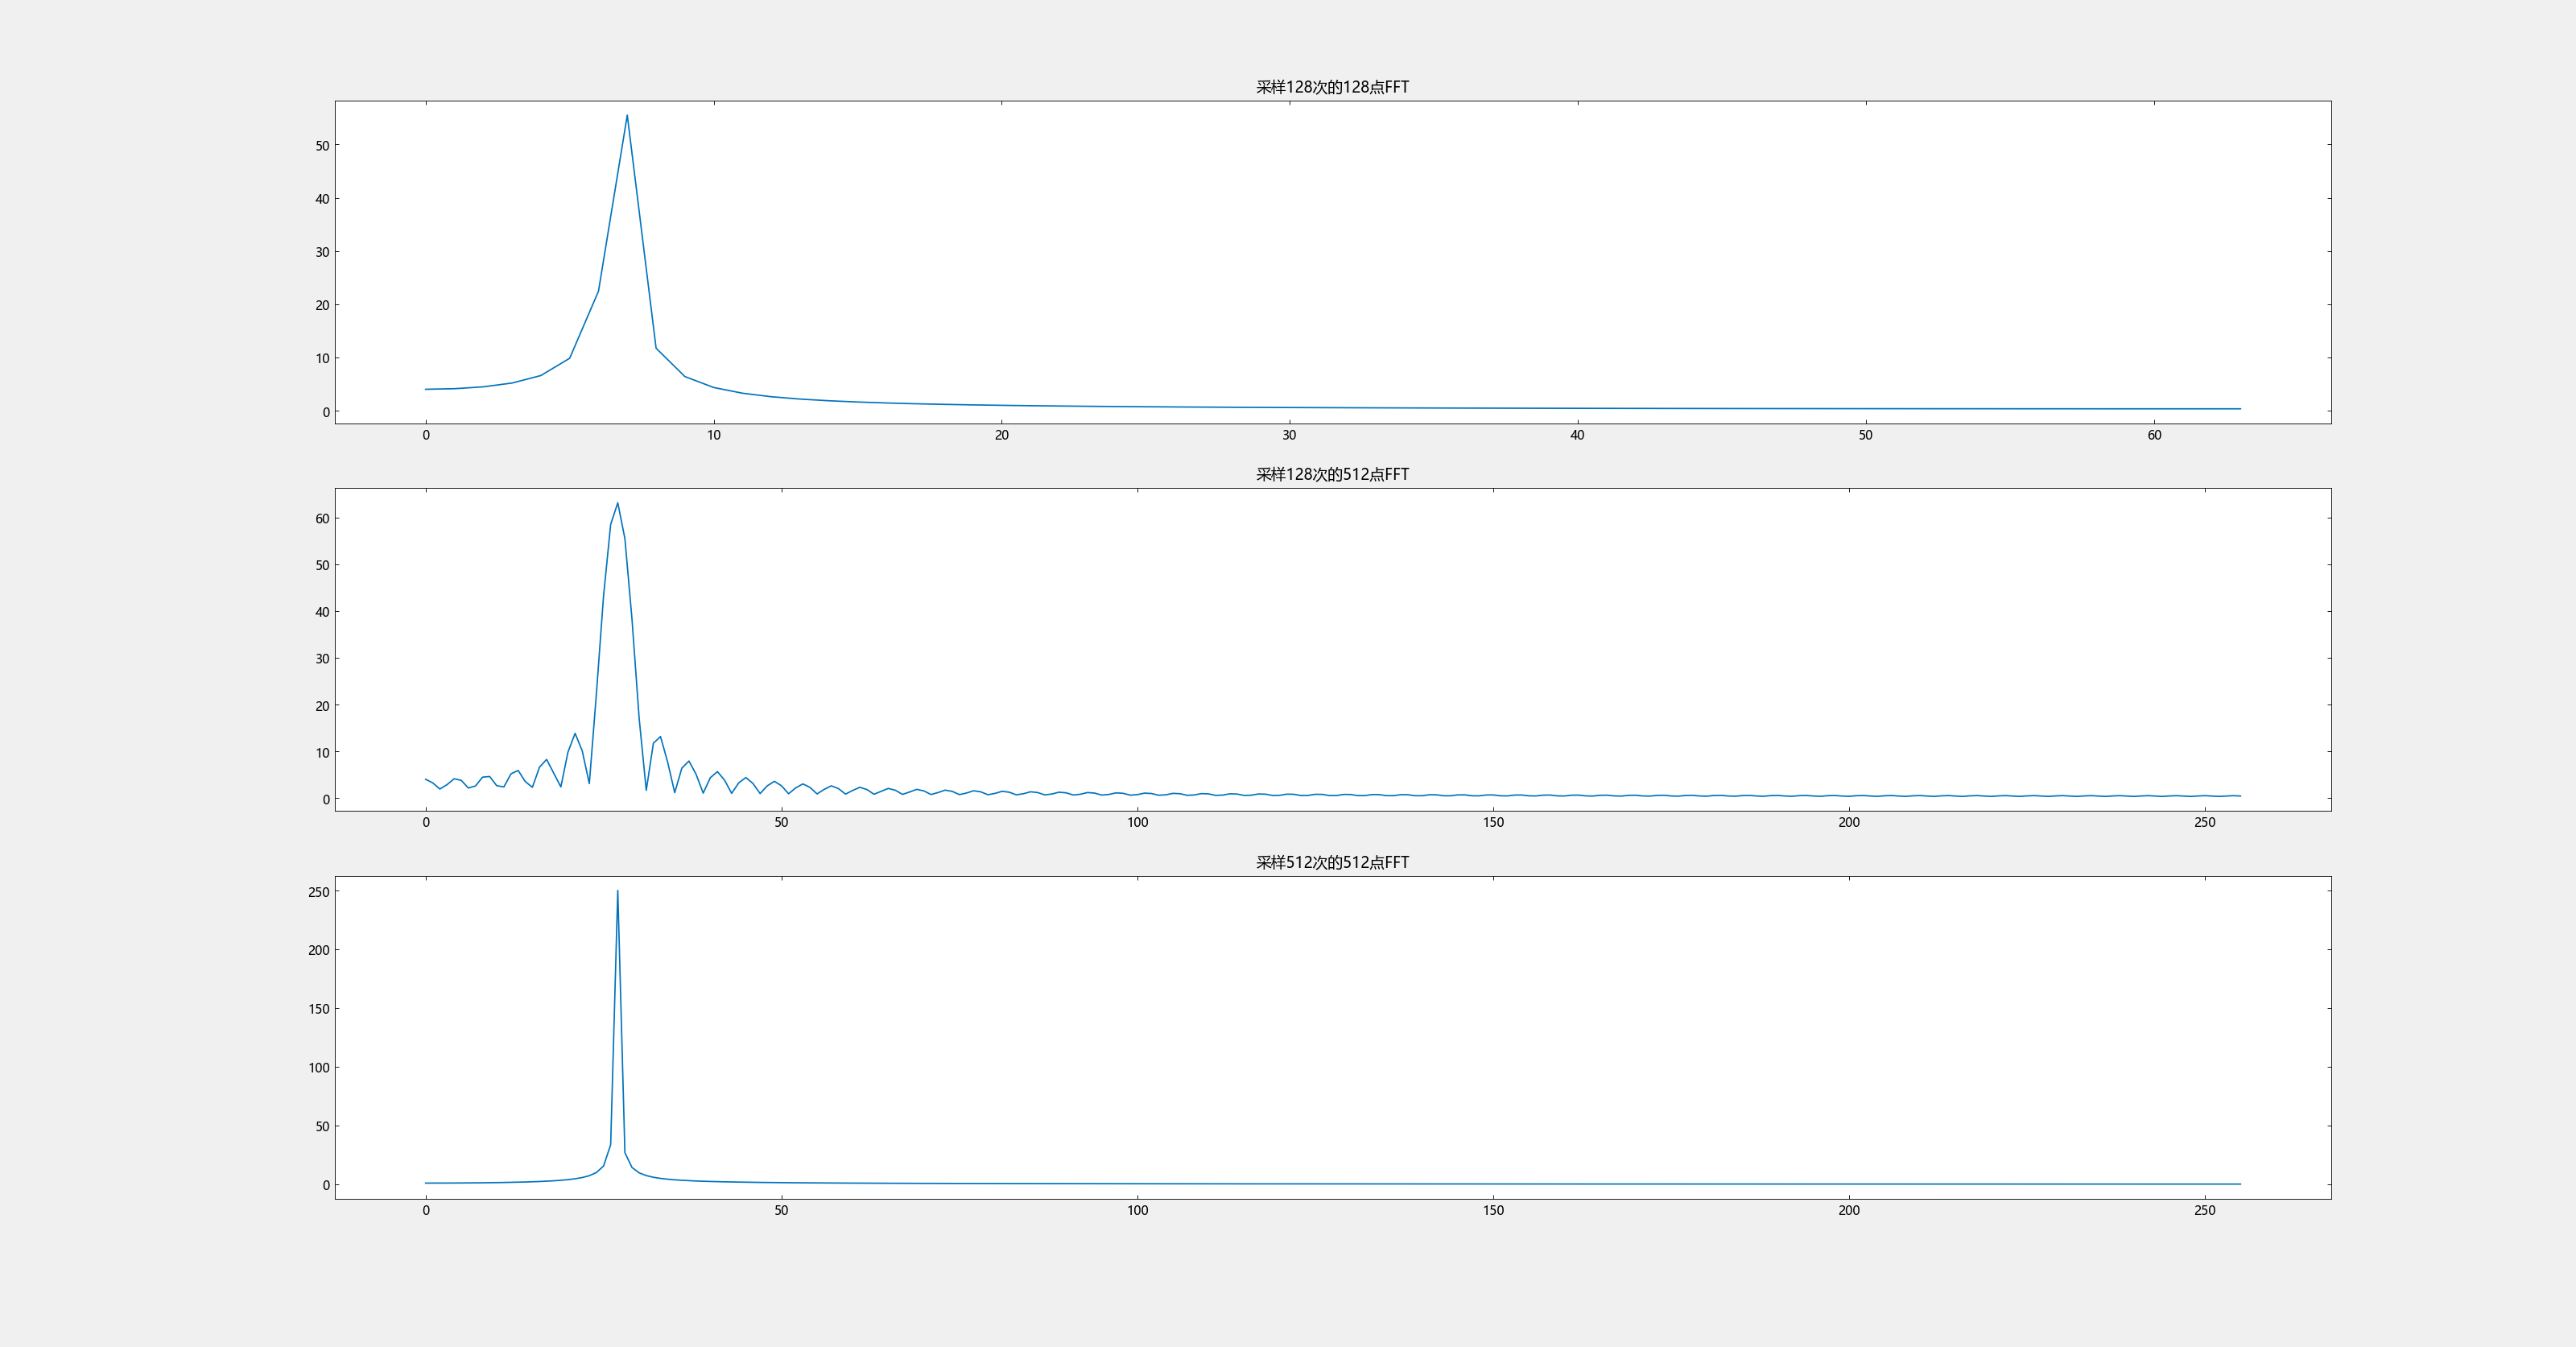
\includegraphics[width=0.75\linewidth]{./图片/第七问}
				\end{subfigure}
				\caption{不同采样点下的采样频谱}
				\label{fig:不同采样点下的采样频谱}
			\end{figure}
		\subsection{结论} 
			  \subsubsection{128点采样，128点FFT}
			频谱分辨率: $\Delta f = f_s/N = 100/128 \approx 0.78125$ Hz
			栅栏效应:频率间隔为 0.78125 Hz，峰值分散至相邻频点（6或7），幅度误差显著。
			\subsubsection{128点采样补零至512点FFT}
			频谱分辨率: 仍为 0.78125 Hz（由原始采样时间决定）\par
			栅栏效应:频率间隔缩小至 $f_s/512 \approx 0.1953 $Hz，但分辨率未提升，误差减小，主瓣展宽导致频谱泄漏。
			
			\subsubsection{512点采样，512点FFT}
			频谱分辨率: $\Delta f = 100/512 \approx 0.1953 Hz$（更高分辨率）\par
			栅栏效应:频率间隔为 0.1953 Hz，间隔更小，误差更小，主瓣更窄。\par
			
			栅栏效应: 由频率间隔决定，补零可减小间隔但无法提高分辨率\par
			频谱分辨率: 仅由采样时间决定，需增加采样点数（非补零）才能提升\par
			最优方案: 512点采样 + 512点FFT，同时提高分辨率并减小栅栏效应
			
	
	
	
	
	\newpage
	\section{系统零极点配置}
		\subsection{题目}
			设计一数字滤波器$y(n)=b_0x(n)+b_1x(n-1)+b_2x(n-2)$滤除窄带频率噪声干扰$f_0=60$Hz,设采样频率为$F_s=300$Hz。
			\begin{compactenum}
				\item 给出约束条件为$H(e^{j0})=1$，确定滤波器系数$b_0$，$b_1$和$b_2$；
				\item 求系统的频率特性，画出频谱图。
			\end{compactenum}
		\subsection{分析}
			滤波器信号为$y(n)=b_0x(n)+b_1x(n-1)+b_2x(n-2)$，经过Z变换得传递函数形式为：
			\begin{align}
				Y(z)&=b_0z^0+b_1z^{-1}+b_2z^{-2}\\
					&\triangleq A(1-x_1z^{-1})(1-x_2z^{-1})
					\label{eq:传递函数}
			\end{align}\par
			为了滤除$f_0=60$Hz的窄带频率噪声干扰，其零点$x_{1,2}$需要满足公式
			\begin{gather}
				x_{1,2}=e^{\pm j\omega_0}
				\label{eq:零点公式}
			\end{gather}
			其中$\omega_0$是滤除信号的数字角频率，满足:
			\begin{gather}
				w_0=\Omega_0 T_s=2\pi f_0\times\frac{1}{F_s}=2\pi \times60\times\frac{1}{300}=\frac{2}{5}\pi
				\label{eq:数字角频率公式}
			\end{gather}\par
			将式\ref{eq:零点公式}和式\ref{eq:数字角频率公式}代入式\ref{eq:传递函数}得：
			\begin{align}
				Y(z)&=A(1-e^{j\frac{2}{5}\pi}z^{-1})(1-e^{-j\frac{2}{5}\pi}z^{-1})\\
				&=A(1-2\cos(\frac{2}{5}\pi)z^{-1}+z^{-2})\\
				&=A(1-\frac{\sqrt{5}-1}{2}z^{-1}+z^{-2})
			\end{align}\par
			由约束条件$H(e^{j0})=1$得：
			\begin{gather}
				Y(e^{j0})=Y(1)=A(1-\frac{\sqrt{5}-1}{2}+1)=\frac{5-\sqrt{5}}{2}A=1
			\end{gather}
			解得：
			\begin{gather}
				A=\frac{5+\sqrt{5}}{10}
			\end{gather}\par
			故最终的滤波器传递函数为：
			\begin{gather}
				Y(z)=\frac{5+\sqrt{5}}{10}z^{0}-\frac{\sqrt{5}}{5}z^{-1}+\frac{5+\sqrt{5}}{10}z^{-2}
			\end{gather}
			滤波器的系数为：
			\begin{gather}
				\begin{cases}
					b_0&=\frac{5+\sqrt{5}}{10}\\
					b_1&=-\frac{\sqrt{5}}{5}\\
					b_2&=\frac{5+\sqrt{5}}{10}
				\end{cases}
			\end{gather}\par
		\subsection{代码}
			\begin{lstlisting}[language=Python]
using TySignalProcessing
using TyMath
using TyPlot 

a=[(5+sqrt(5))/10,-sqrt(5)/5,(5+sqrt(5))/10]    # 数字滤波器分子部分
b=[1]                                           # 数字滤波器分母部分
h,f = freqz(a,b,512,300)        # 得到512个采样点下采样速率为300Hz数字滤波器的频率响应向量h和相应的频率向量f
plot(f,20*log10.(abs.(h)))      # 绘制频率响应曲线
xlabel("归一化数字频率f0/Hz")    # 给出x轴标题
ylabel("幅度/dB")               # 给出y轴标题
			\end{lstlisting}
		\subsection{运行结果}
			\begin{figure}[H]
				\centering
				\begin{subfigure}{\linewidth}
					\centering
					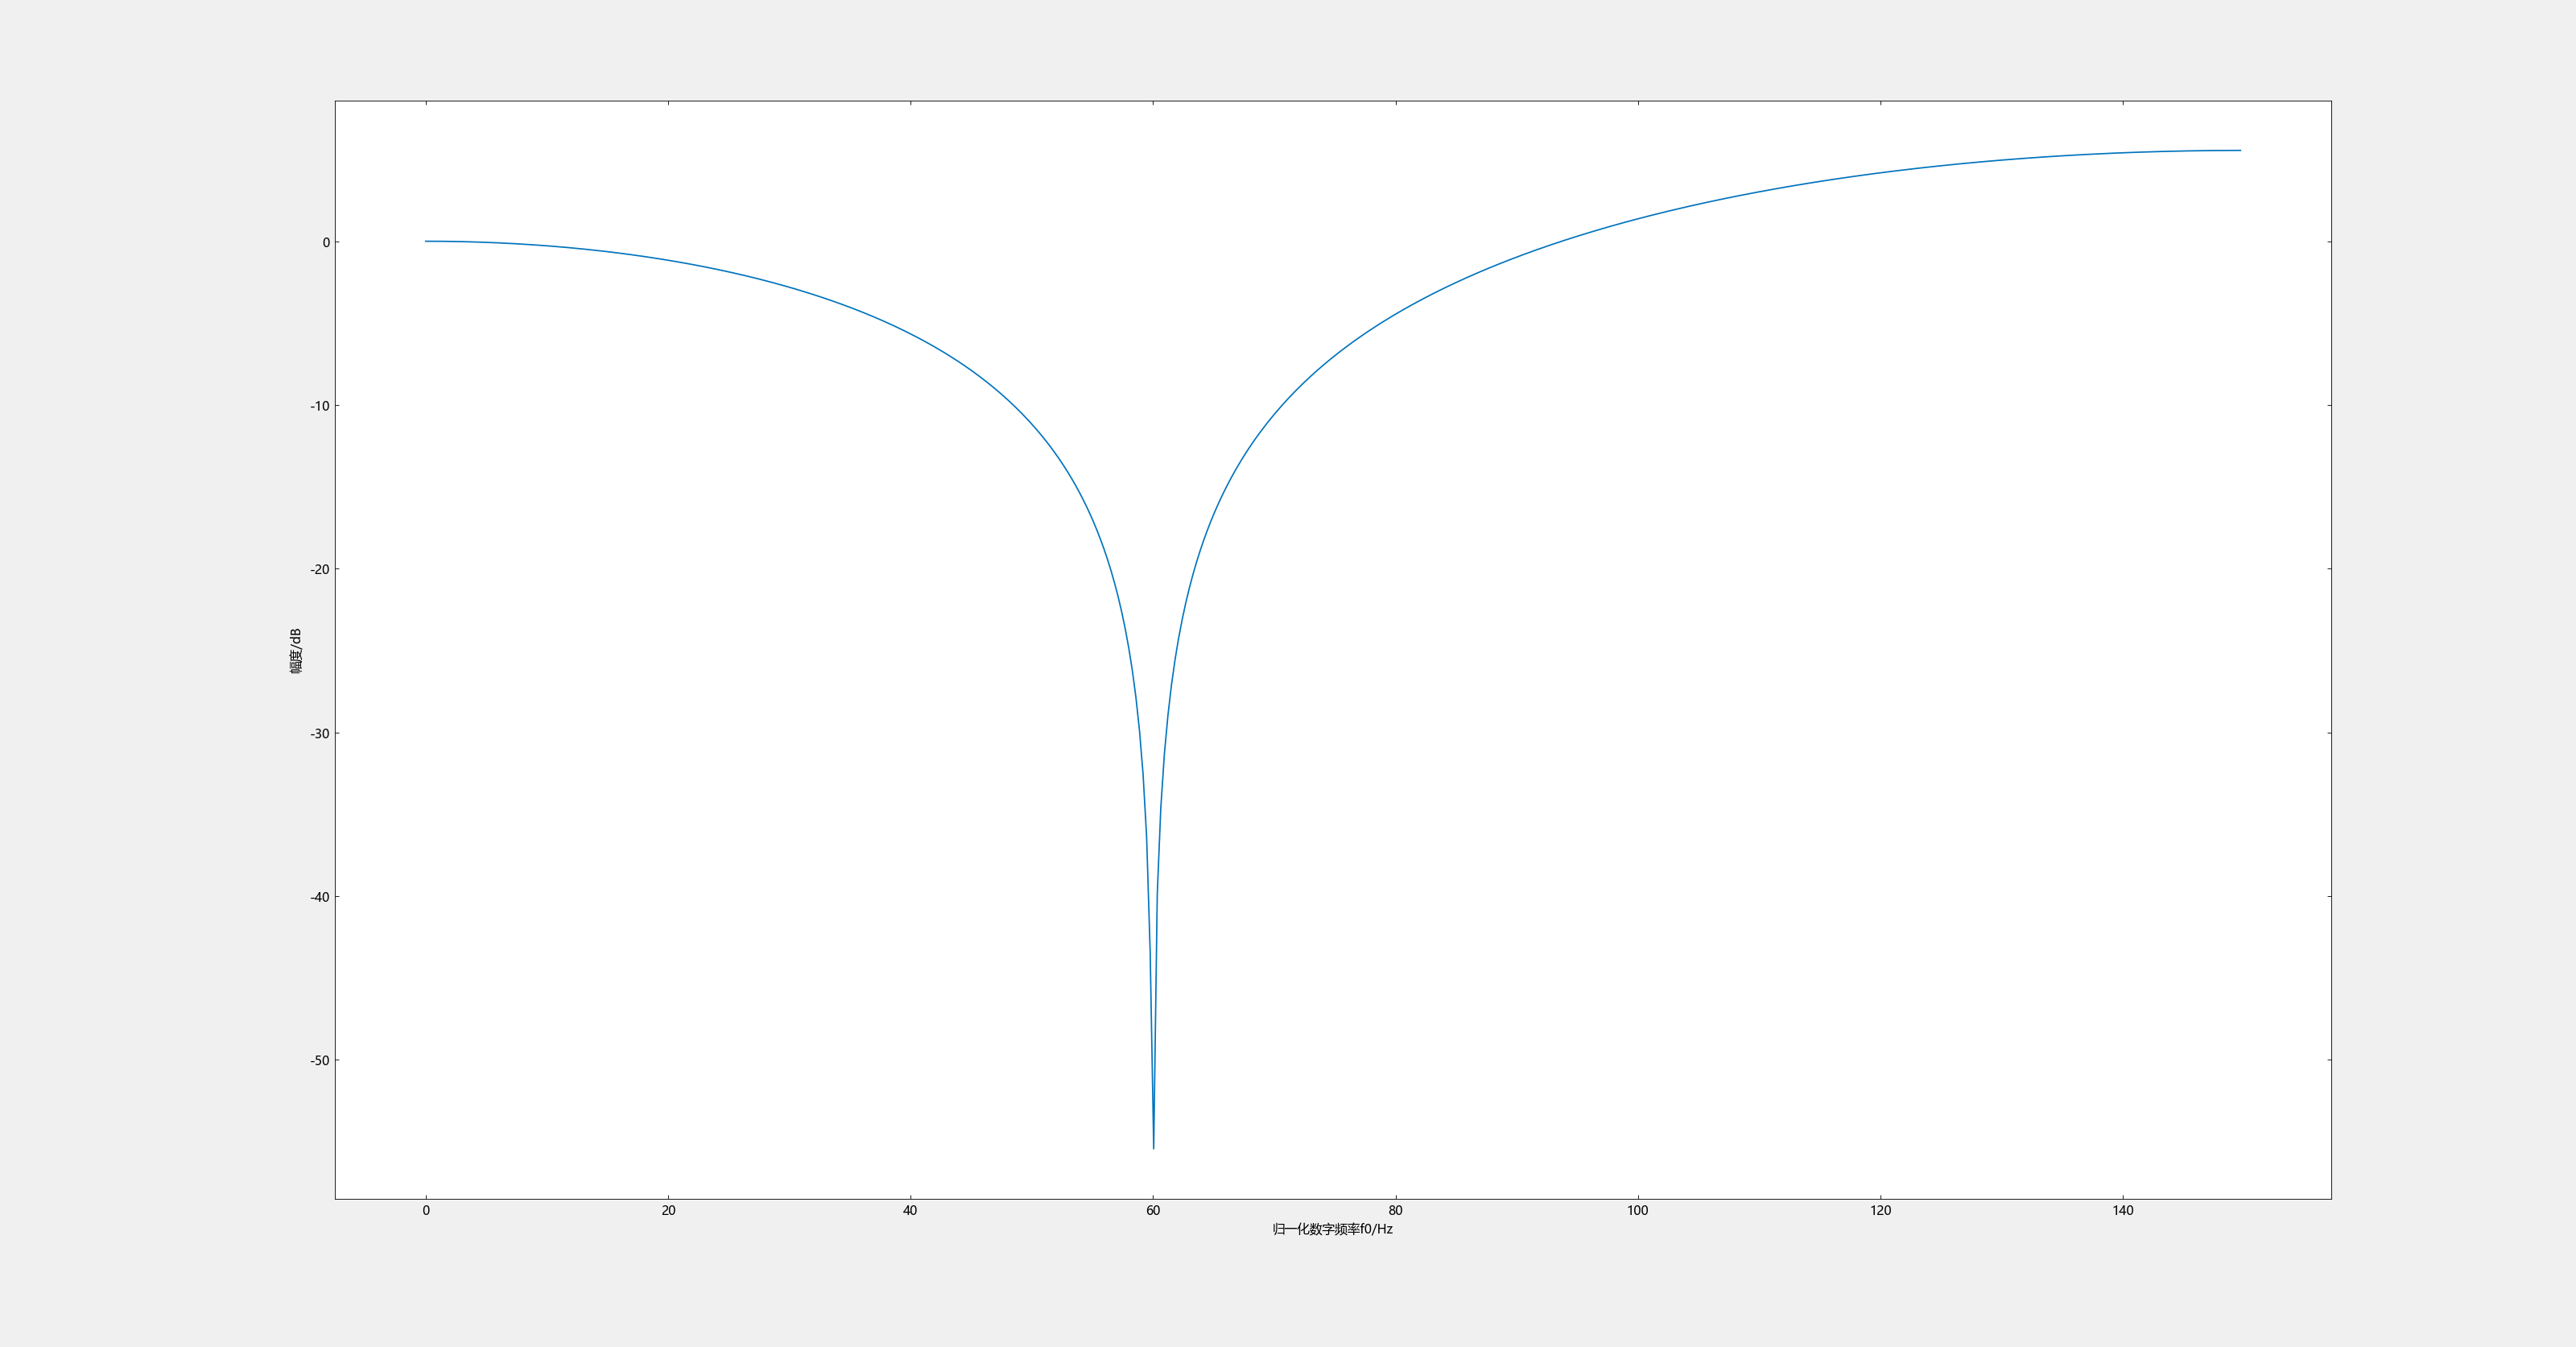
\includegraphics[width=0.55\linewidth]{./图片/第八问}
				\end{subfigure}
				\caption{滤波器幅频特性}
				\label{fig:滤波器幅频特性}
			\end{figure}
		\subsection{结论}
			由图\ref{fig:滤波器幅频特性}观察可得，60Hz处出现深凹（陷波），表明噪声被滤除。直流增益为0dB（即增益=1），符合设计约束。其他频率信号基本无衰减（如30Hz或90Hz）。
			
	\newpage
	\section{窗函数比较}
		\subsection{题目}
			完成矩形窗、三角窗、汉宁窗、汉明窗等窗口函数的时域波形与频谱并做简要分析。
		\subsection{代码}
			\begin{lstlisting}[language=Python]
using TySignalProcessing
using TyMath
using TyPlot 
# 定义频率响应绘图函数plot_freqz，其中w为窗函数采样点，i为子图数
function plot_freqz(w,i)
h,a=freqz(w)                    # 得到512个采样点下频率响应向量h和相应的频率向量f
subplot(2,4,i)                  # 在第i张子图上绘制
plot(a/pi,20*log10.(abs.(h)))   # 绘制频率响应曲线
xlabel("归一化数字角频率")       # 给出x轴标题
ylabel("幅度/dB")               # 给出y轴标题
end

###  矩形窗绘制部分  ###
subplot(2,4,1)                      # 在第1张子图上绘制
w = rectwin(51)                     # 给出51点的矩形窗函数波形
plot(w);title("矩形窗")             # 绘制时域波形并给出标题
plot_freqz(w,5)                     # 绘制频谱

###  三角窗绘制部分  ###
subplot(2,4,2)                      # 在第2张子图上绘制
w = triang(51)                     # 给出51点的三角窗函数波形
plot(w);title("三角窗")             # 绘制时域波形并给出标题
plot_freqz(w,6)                     # 绘制频谱

###  汉宁窗绘制部分  ###
subplot(2,4,3)                      # 在第3张子图上绘制
w = hann(51)                        # 给出51点的汉宁窗函数波形
plot(w);title("汉宁窗")             # 绘制时域波形并给出标题
plot_freqz(w,7)                     # 绘制频谱

###  汉明窗绘制部分  ###
subplot(2,4,4)                      # 在第4张子图上绘制
w = hamming(51)                     # 给出51点的汉明窗函数波形
plot(w);title("汉明窗")             # 绘制时域波形并给出标题
plot_freqz(w,8)                     # 绘制频谱
			\end{lstlisting}
		\subsection{运行结果}
			\begin{figure}[H]
				\centering
				\begin{subfigure}{\linewidth}
					\centering
					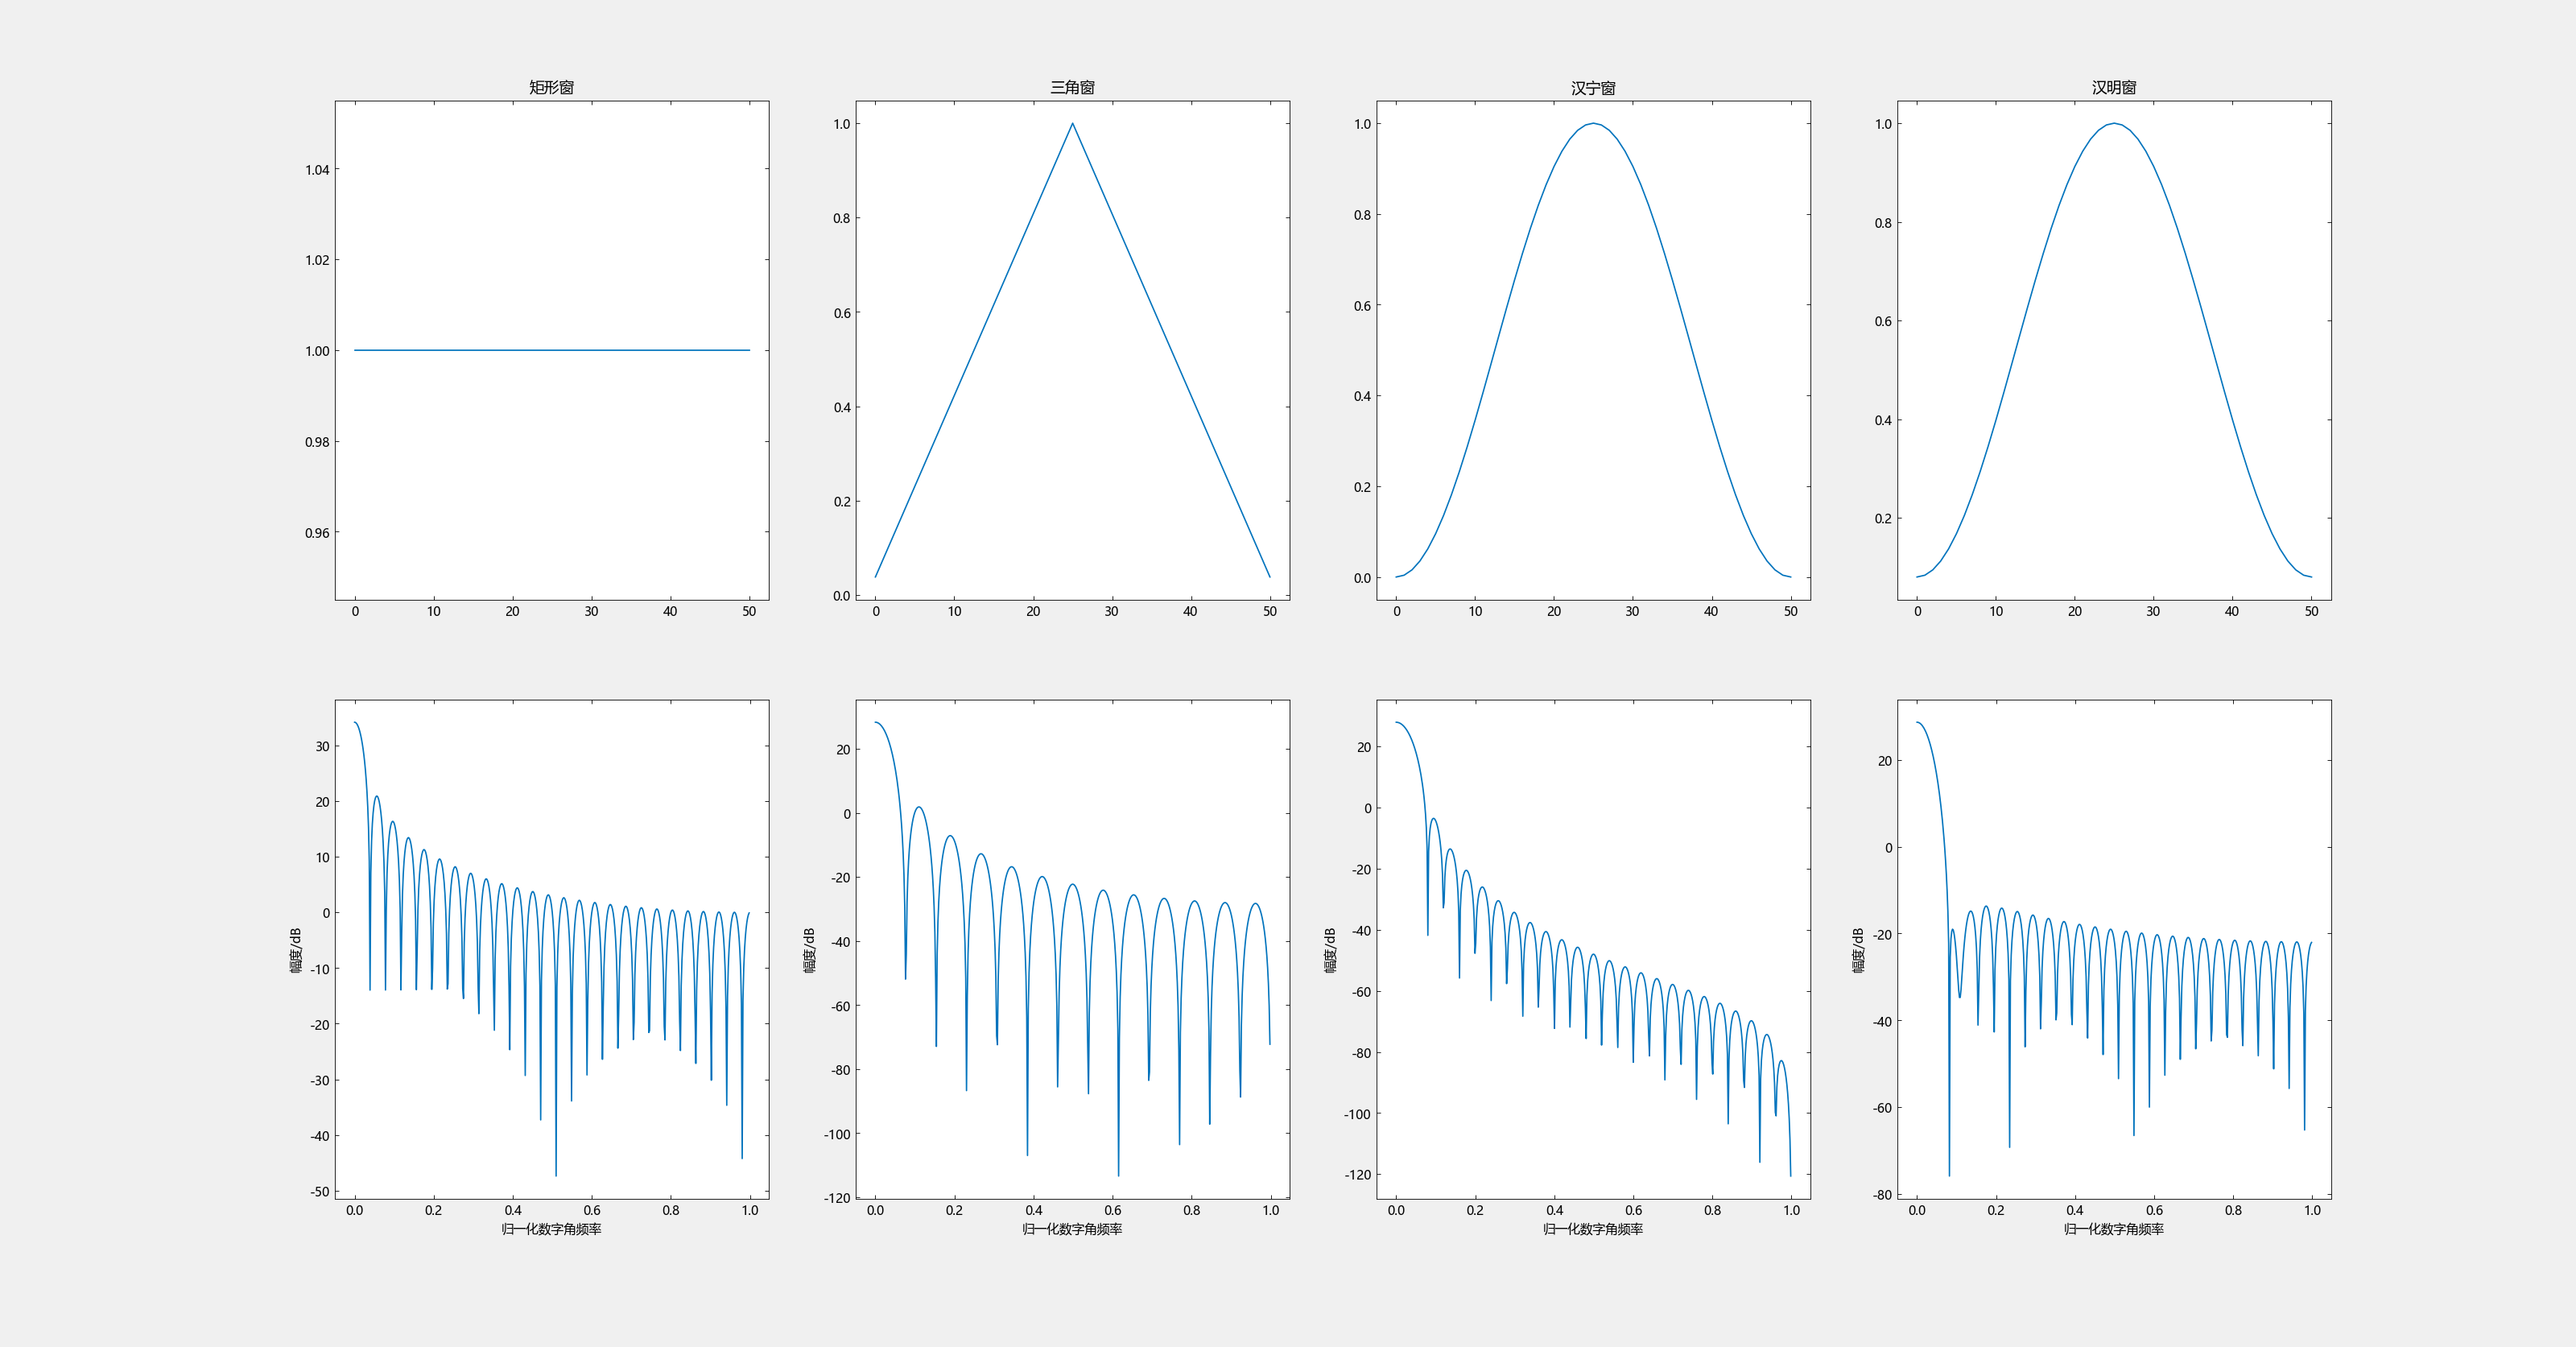
\includegraphics[width=0.55\linewidth]{./图片/第九问}
				\end{subfigure}
				\caption{窗口函数的时域波形与频谱}
				\label{fig:窗口函数的时域波形与频谱}
			\end{figure}
		\subsection{结论}
			\subsubsection{矩形窗}
				表达式：$w(n)=R_n(n)$\par
				频率响应为：$W_R(e^{j\omega})=\frac{\sin(\omega N/2)}{\sin(\omega /2)}e^{-j \frac{N-1}{2}\omega}$\par
				频谱图特点：最简单的窗口，在有效区间内取值为1，两端无平滑过渡。\par
				频谱特性：其中$W_R (e^{j\omega})$主瓣宽度为$\frac{4\pi}{N}$，第一旁瓣比主瓣低$13$dB，最小阻带衰减$21$dB。
			\subsubsection{三角窗}
				表达式：$w(n)=1-\frac{2\lvert n-(N-1)/2\rvert}{N-1}$\par
				频谱图特点：呈三角形，两端线性递减到$0$，中间最高。\par
				频谱特性：主瓣宽度比矩形窗宽（约$\frac{8\pi}{N}$）。第一旁瓣峰值约$-27$dB，比主瓣低$26$dB，最小阻带衰减$25$dB。
			\subsubsection{汉宁窗}
				表达式：$w(n)=0.5-0.5\cos⁡\frac{2\pi n}{N-1}$\par
				频谱图特点：余弦平方形状，两端平滑过渡到$0$，中间较高。\par
				频谱特性：主瓣宽度约$\frac{8\pi}{N}$。第一旁瓣峰比主瓣约低$31$dB，最小阻带衰减$44$dB。
			\subsubsection{汉明窗}
				表达式：$w(n)=0.54-0.46\cos⁡\frac{2\pi n}{N-1}$\par
				频谱图特点：类似汉宁窗，但两端不完全归零，起始/结束值为0.08。\par
				频谱特性：可将99.96\%的能量集中在窗谱的主瓣内，主瓣宽度与汉宁窗相同（约$\frac{8\pi}{N}$）。第一旁瓣峰比主瓣约低$41$dB，最小阻带衰减$53$dB。
			
	
	\newpage
	\section{滤波器设计}
		\subsection{题目}
			\begin{compactenum}
				\item 完成IIR模拟低通滤波器设计并分别采用脉冲响应不变法与双线性法转换成数字滤波器。通带0 - 4 kHz，通带最大衰减-2dB，阻带 > 5kHz，衰减至少-40dB，采样频率20kHz
				\item 完成FIR数字低通滤波器设计通带0 - 4 kHz，阻带 > 5kHz，衰减至少-40dB，采样频率20kHz。
			\end{compactenum}
		\subsection{设计分析}
			\subsubsection{模拟低通滤波器设计}
				 根据题目能够确定模拟滤波器指标：
				 \begin{compactitem}
				 	\item 通带截止频率$f_p=4$kHz
				 	\item 阻带起始频率$f_s=5$kHz
				 	\item 通带最大衰减$\alpha_p=2$dB
				 	\item 阻带最小衰减$\alpha_s=40$dB
				 \end{compactitem}
				 则通带截止角频率$\Omega_p=4000\times2\times\pi=8000\pi$，阻带起始角频率$\Omega_s=5000\times2\times\pi=10000\pi$。\par
				 设计巴特沃斯低通滤波器，首先计算阶数$N$及3dB截止频率$\Omega_c$。
				 \begin{gather}
				 	\lambda_{sp}=\frac{\Omega_s}{\Omega_p}=\frac{10000\pi}{8000\pi}=1.25\\
				 	k_{sp}=\sqrt{\frac{10^{0.1\alpha_p}-1}{10^{0.1\alpha_s}-1}}=0.007648\\
				 	N=\frac{\lg k_{sp}}{\lg \lambda_{sp}}=-\frac{\lg 0.007648}{\lg 1.25}=21.83935\\
				 	\Omega_c=\Omega_p(10^{0.1\alpha_p}-1)^{-\frac{1}{2N}}=8000\pi(10^{0.1\times2}-1)^{-\frac{1}{2\times22}}=25440.96
				 \end{gather}
				取$N=22$，得归一化传递函数为：
				\begin{gather}
					H(p)=\prod_{k=0}^{10}\frac{1}{p^2+2\cos(\frac{2k+1}{2N}\pi)p+1}
					\label{eq:归一化传递函数}
				\end{gather}
				为去归一化，将$p=s/\Omega_c$代入式\ref{eq:归一化传递函数}中，得到实际的传递函数
				\begin{align}
					H(s)&=\prod_{k=0}^{10}\frac{\Omega_c^2}{s^2+2\cos(\frac{2k+1}{2N}\pi)\Omega_c s+\Omega_c^2}\\aw
						&=\prod_{k=0}^{10}\frac{6.4734\times 10^8}{s^2+20881.93\cos(\frac{2k+1}{44}\pi) s+6.4734\times 10^8}
					\label{eq:实际传递函数}
				\end{align}
			\subsubsection{IIR数字低通滤波器}
				将式\ref{eq:实际传递函数}做Z变换，可以直接得到对应的IIR数字低通滤波器。
				\begin{figure}[H]
					\centering
					\begin{subfigure}{\linewidth}
						\centering
						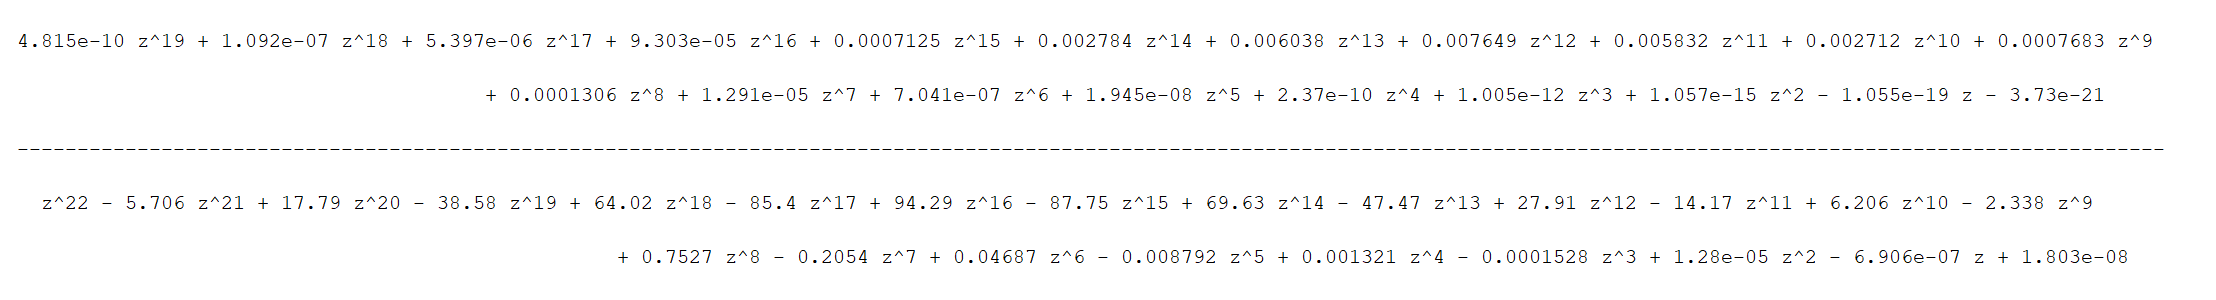
\includegraphics[width=0.95\linewidth]{aa}
					\end{subfigure}
				\end{figure}
			\subsubsection{FIR数字低通滤波器}
				计算对应数字频率：通带截止频率为
				\begin{gather}
					\omega_p=2\pi\frac{\Omega_p}{\Omega_s}=0.4\pi
				\end{gather}
				阻带起始频率为
				\begin{gather}
					\omega_{st}=2\pi\frac{\Omega_{st}}{\Omega_s}=0.5\pi
				\end{gather}\par
				设$H_d(e^{j\omega})$为理想的线性相位低通滤波器。
				\begin{gather}
					H_d(e^{j\omega})=
					\begin{cases}
						e^{-j\omega\alpha},&\lvert \omega \rvert\leq \omega_c\\
						0,&\omega_c<\lvert \omega \rvert\leq\pi
					\end{cases}
				\end{gather}
				首先由所需低通滤波器的过渡带求理想滤波器的截止频率$\Omega_c$
				\begin{gather}
					\Omega_c\approx\frac{1}{2}(\Omega_p+\Omega_{st})=2\pi\times4.5\times10^3
				\end{gather}
				对应的数字频率为
				\begin{gather}
					\omega_c=2\pi\frac{\Omega_c}{\Omega_s}=0.45\pi
				\end{gather}
				由此可得
				\begin{gather}
					h_d(n)=\frac{1}{2\pi}\int_{-\omega_c}^{\omega_c}e^{-j\omega\alpha}e^{j\omega n}d\omega=\frac{\sin[\omega_c(n-\alpha)]}{\pi(n-\alpha)}
				\end{gather}			
				式中，$\alpha=\frac{N-1}{2}$，保证滤波器的线性相位。
				由于要求阻带衰减不小于40dB，可选用哈明窗，其阻带最小衰减为-53dB，满足要求。所要求的过渡带宽$\Delta\omega=\omega_{st}-\omega_p=0.1\pi$，因哈明窗过渡带宽满足$\Delta\omega=8\pi/N$，所以
				\begin{gather}
					N=\frac{8\pi}{\Delta\omega}=80
				\end{gather}
				取$N=81$，则
				\begin{gather}
					\alpha=\frac{N-1}{2}=40
				\end{gather}\par
				由哈明窗表达式$w(n)$确定FIR滤波器的$h(n)$：
				\begin{gather}
					w_{Hm}(n)=[0.54-0.46\cos(\frac{2\pi n}{N-1})]w_R(n)\\
					h_d(n)=\frac{\sin[\omega_c(n-\frac{N-1}{2})]}{\pi(n-\frac{N-1}{2})}\\
					H(n)=h_d(n)w(n)=\frac{\sin0.45\pi(n-40)}{\pi(n-40)}(0.54-0.46\cos(\frac{\pi n}{40}))w_R(n)
				\end{gather}	
				
	
			
			
			
			
			
			
			
			
			
			
			
			
			
			
			
			
			
			
			
			
			
			
			
			
			
\end{document}




